\documentclass{article}
\usepackage{tikz}
\usetikzlibrary{calc}
\usepackage{amsmath}
\usepackage[paperwidth=40cm,paperheight=22cm,margin=0pt]{geometry}
\pagestyle{empty}
\begin{document}
\centering
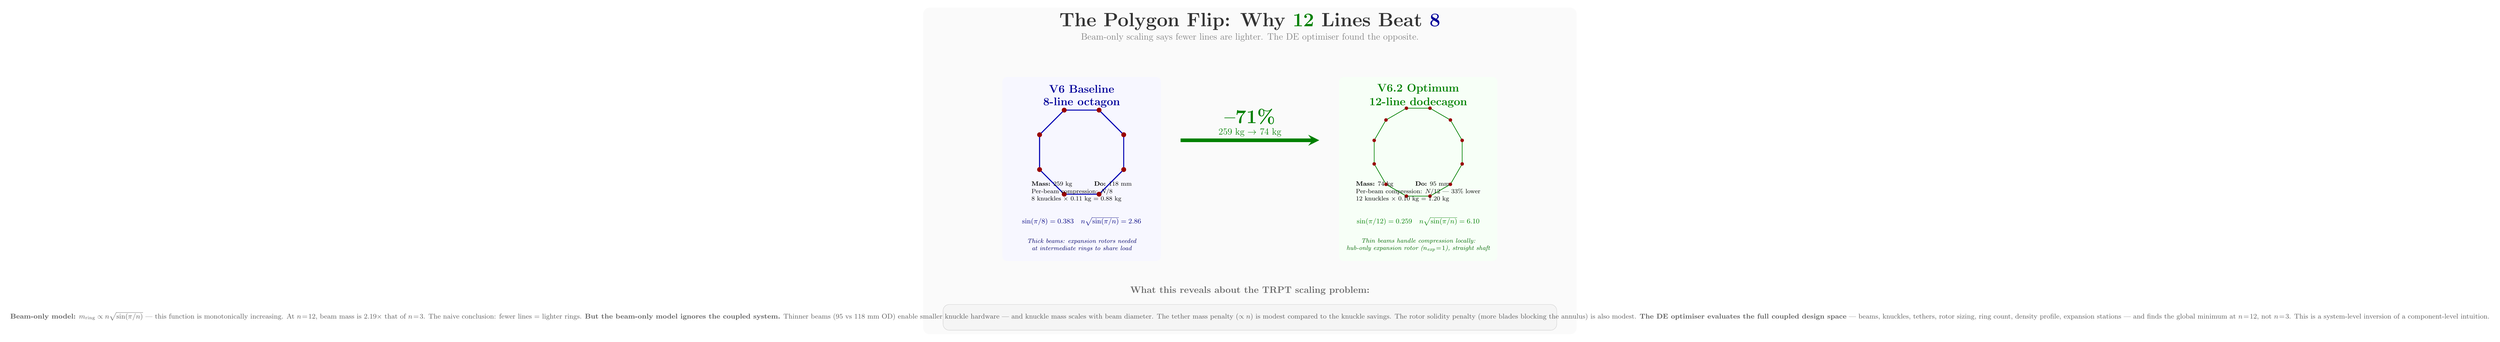
\begin{tikzpicture}[scale=0.90]

% Background
\fill[black!2, rounded corners=8pt] (-16.5,-9.0) rectangle (16.5,7.5);

% === TITLE ===
\node[font=\bfseries\Huge, black!80] at (0,6.8) {The Polygon Flip: Why {\color{green!50!black} 12} Lines Beat {\color{blue!60!black} 8}};
\node[font=\large, black!50] at (0,6.0) {Beam-only scaling says fewer lines are lighter. The DE optimiser found the opposite.};

% === LEFT: OCTAGON ===
\begin{scope}[xshift=-8.5cm, yshift=0.2cm]
  \fill[blue!3, rounded corners=6pt] (-4.0,-5.5) rectangle (4.0,3.8);
  \node[font=\bfseries\Large, blue!60!black] at (0,3.2) {V6 Baseline};
  \node[font=\Large\bfseries, blue!60!black] at (0,2.5) {{\Large 8}-line octagon};

  \foreach \i in {1,...,8} {
    \coordinate (O\i) at ({2.3*cos(360*\i/8 + 22.5)}, {2.3*sin(360*\i/8 + 22.5)});
  }
  \draw[blue!70!black, line width=1.3pt] (O1) -- (O2) -- (O3) -- (O4) -- (O5) -- (O6) -- (O7) -- (O8) -- cycle;
  \foreach \i in {1,...,8} { \fill[red!60!black] (O\i) circle (3.5pt); }

  \node[font=\footnotesize, align=left] at (0,-2.0) {
    \textbf{Mass:} 259 kg \hspace{0.8cm} \textbf{Do:} 118 mm\\
    Per-beam compression: $N/8$\\
    8 knuckles $\times$ 0.11 kg = 0.88 kg};
  \node[font=\small, blue!50!black] at (0,-3.5) {$\sin(\pi/8)=0.383$\quad $n\sqrt{\sin(\pi/n)}=2.86$};
  \node[font=\footnotesize\itshape, blue!40!black, align=center] at (0,-4.7) {Thick beams: expansion rotors needed\\at intermediate rings to share load};
\end{scope}

% === ARROW ===
\draw[->, line width=5pt, >=stealth, green!50!black] (-3.5,0.8) -- (3.5,0.8);
\node[font=\bfseries\Huge, green!50!black] at (0,2.0) {\textbf{--71\%}};
\node[font=\large, green!50!black] at (0,1.2) {259 kg $\rightarrow$ 74 kg};

% === RIGHT: DODECAGON ===
\begin{scope}[xshift=8.5cm, yshift=0.2cm]
  \fill[green!3, rounded corners=6pt] (-4.0,-5.5) rectangle (4.0,3.8);
  \node[font=\bfseries\Large, green!50!black] at (0,3.2) {V6.2 Optimum};
  \node[font=\Large\bfseries, green!50!black] at (0,2.5) {{\Large 12}-line dodecagon};

  \foreach \i in {1,...,12} {
    \coordinate (D\i) at ({2.3*cos(360*\i/12 + 15)}, {2.3*sin(360*\i/12 + 15)});
  }
  \draw[green!50!black, line width=0.8pt] (D1) foreach \i in {2,...,12} { -- (D\i) } -- cycle;
  \foreach \i in {1,...,12} { \fill[red!60!black] (D\i) circle (2.5pt); }

  \node[font=\footnotesize, align=left] at (0,-2.0) {
    \textbf{Mass:} 74 kg \hspace{0.8cm} \textbf{Do:} 95 mm\\
    Per-beam compression: $N/12$ --- 33\% lower\\
    12 knuckles $\times$ 0.10 kg = 1.20 kg};
  \node[font=\small, green!50!black] at (0,-3.5) {$\sin(\pi/12)=0.259$\quad $n\sqrt{\sin(\pi/n)}=6.10$};
  \node[font=\footnotesize\itshape, green!40!black, align=center] at (0,-4.7) {Thin beams handle compression locally:\\
  hub-only expansion rotor ($n_{\text{exp}}\!=\!1$), straight shaft};
\end{scope}

% === FINDINGS BOX (below both diagrams) ===
\fill[black!4, draw=gray!40, rounded corners=8pt] (-15.5,-7.5) rectangle (15.5,-8.8);
\node[font=\bfseries\large, black!60] at (0,-6.8) {What this reveals about the TRPT scaling problem:};

\node[font=\small, align=left, black!65] at (0,-8.1) {
  \textbf{Beam-only model:} $m_{\text{ring}} \propto n\sqrt{\sin(\pi/n)}$ — this function is monotonically increasing. At $n\!=\!12$, beam mass is $2.19\times$ that of $n\!=\!3$.
  The naive conclusion: fewer lines = lighter rings. \textbf{But the beam-only model ignores the coupled system.} Thinner beams (95 vs 118 mm OD) enable
  smaller knuckle hardware — and knuckle mass scales with beam diameter. The tether mass penalty ($\propto n$) is modest compared to the knuckle savings.
  The rotor solidity penalty (more blades blocking the annulus) is also modest. \textbf{The DE optimiser evaluates the full coupled design space} — beams, knuckles,
  tethers, rotor sizing, ring count, density profile, expansion stations — and finds the global minimum at $n\!=\!12$, not $n\!=\!3$. This is a system-level
  inversion of a component-level intuition.};

\end{tikzpicture}
\end{document}
